\chapter{Results}\label{cha:results}

In this chapter, the results of the experiments are reported, as described in \Cref{cha:methods}. Some sentences and formulations are adapted from the project report \textit{Multi-layer Perceptrons for Branching in Mixed-Integer Linear Programming} (2020), as this thesis shares methods with the aforementioned report. 


\section{Data Set}\label{sec:datagen}

Problem instances are generated as described in \Cref{ssec:probleminstances}. In total, $2000$ training instances, $500$ validation instances, and $ 500 $ test instances are created. These are of size $100 \times 500$ for the combinatorial auction problems and $100 \times 500$ for the set covering problems, as stated in \Cref{sec:dataset}. This information is shown in \Cref{tab:instances}.

The generated problem instances are then solved as specified in \Cref{ssec:expertsolutiongeneration}. This results in a total of 50000 training samples, 10000 validation samples, and 10000 test samples for the combinatorial auctions problems, and the same for the set covering problems. This is also shown in \Cref{tab:instances}.

The division into train, validation and test sets is done as is standard in \gls{ML} development \cite{goodfellow2016deep}. The train set will be used to optimize the model parameters, the validation set will be used to monitor the model's ability to generalize to unseen samples, and the test set will be used to evaluate the model. 

A notable difference between the problem classes is the number of constraints. The combinatorial auction problems average about 200 constraints, while the set covering problems have 500 constraints.  

$250$ problem instances are generated for evaluating the efficiency of the models. %In addition, as is done in \cite{gasse2019exact}, additional larger problems are generated in order to evaluate the models' ability to perform on more difficult problems. This includes $50$ medium-sized instances and $20$ large-sized instances. These problems are shown in \Cref{tab:samp_transf}.

\begin{scriptsize}
\begin{table}[ht]
	\centering
	\begin{tabular}{llccc}
		\toprule
		  && \multicolumn{1}{c}{Train} & \multicolumn{1}{c}{Validate} & \multicolumn{1}{c}{Test}\\
		  \cmidrule(lr){3-3} \cmidrule(lr){4-4} \cmidrule(lr){5-5}
		  \multirow{3}{*}{Auctions} & Dimensions & $100 \times 500$ & $100 \times 500$ & $100 \times 500$ \\
		% \midrule
		& Instances & 2000 &  500  & 250\\
		& Samples & 50000 &  10000  & 10000 \\
		\addlinespace
		\multirow{3}{*}{Setcover} & Dimensions & $500\times1000$ & $500\times1000$ & $500\times1000$\\
		% \midrule
		 & Instances & 2000 &  500  & 500 \\
		 & Samples & 50000 &  10000  & 50000 \\
		% \addlinespace
		\bottomrule
	\end{tabular}
	\caption{Data set, dimensions and number of problem instances for each problem class.}\label{tab:instances}
\end{table}
\end{scriptsize}

\begin{comment}
  \begin{scriptsize}
\begin{table}[ht]
	\centering
	\begin{tabular}{llccc}
		\toprule
		&& \multicolumn{1}{c}{Small} & \multicolumn{1}{c}{Medium} & \multicolumn{1}{c}{Large}\\
		  \cmidrule(lr){3-3} \cmidrule(lr){4-4} \cmidrule(lr){5-5}
		  \multirow{2}{*}{Auctions} & Dimensions & $100 \times 500$ & $200 \times 1000$ & $300 \times 1500$ \\
		% \midrule
		& Instances & 250 &  50  & 20\\
		\addlinespace
		\multirow{2}{*}{Setcover} & Dimensions & $500\times1000$ & $1000\times1000$ & $2000\times1000$\\
		% \midrule
		 & Instances & 250 &  50  & 20 \\
		% \addlinespace
		\bottomrule
	\end{tabular}
	\caption{Data set, dimensions and number of problem instances for each problem class.}\label{tab:samp_transf}
\end{table}
\end{scriptsize}
  
\end{comment}




\section{Training}\label{sec:res_training}

The training was performed as described in \Cref{sec:trainingprotocol}. 
The training graph for MLP2 on the combinatorial auction data set is shown in \Cref{fig:training_mlp2}, and the training graph for GNN1 on the set covering data set is shown in \Cref{fig:training_gnn1}. The Training and validation loss quickly converges before flattening out. There is no discernible difference between training and validation loss. Loss graphs for the other models are not presented, as they are very similar, and are therefore considered to be of little interest. 
%

\begin{figure}[ht]
    \begin{tikzpicture}
      \begin{axis}[
        mlineplot,
        ylabel={Logloss},
        xlabel={Epoch},
        width=\textwidth,
        height=7cm,
	    ymin=2.95,   ymax=3.1,
	    xtick=data,
	    legend style={at={(0.01,0.9)},anchor=west},
	    cycle list name=black white,
	    minor xtick={1, 2, ..., 55},
        xtick={0, 5, ..., 55},
        ytick={2.9, 2.95, ..., 4.4},
      ]
        \addplot plot coordinates{(1, 4.095) (2, 3.315) (3, 3.015) (4, 3.008) (5, 3.003) (6, 3.0) (7, 2.995) (8, 2.991) (9, 2.987) (10, 2.985) (11, 2.984) (12, 2.982) (13, 2.982) (14, 2.981) (15, 2.98) (16, 2.98) (17, 2.979) (18, 2.979) (19, 2.979) (20, 2.978) (21, 2.978) (22, 2.978) (23, 2.978) (24, 2.977) (25, 2.977) (26, 2.977) (27, 2.976) (28, 2.976) (29, 2.975) (30, 2.976) (31, 2.976) (32, 2.975) (33, 2.975) (34, 2.974) (35, 2.975) (36, 2.974) (37, 2.974) (38, 2.974) (39, 2.974) (40, 2.974) (41, 2.973) (42, 2.973) (43, 2.973) (44, 2.973) (45, 2.974) (46, 2.973) (47, 2.97) (48, 2.97) (49, 2.969) (50, 2.969) (51, 2.969) (52, 2.969) (53, 2.969) (54, 2.969) (55, 2.969)};
        \addplot plot coordinates{(1, 4.095) (2, 3.031) (3, 3.019) (4, 3.011) (5, 3.011) (6, 3.005) (7, 3.002) (8, 3.004) (9, 3.009) (10, 3.002) (11, 2.995) (12, 3.002) (13, 2.997) (14, 2.996) (15, 2.997) (16, 2.996) (17, 2.998) (18, 2.995) (19, 2.996) (20, 2.996) (21, 2.993) (22, 2.996) (23, 2.997) (24, 2.994) (25, 2.994) (26, 2.996) (27, 2.996) (28, 2.991) (29, 2.995) (30, 2.999) (31, 2.995) (32, 2.995) (33, 2.994) (34, 2.995) (35, 2.99) (36, 2.991) (37, 2.995) (38, 2.991) (39, 2.994) (40, 2.992) (41, 2.994) (42, 2.993) (43, 2.991) (44, 2.991) (45, 2.992) (46, 2.991) (47, 2.991) (48, 2.991) (49, 2.991) (50, 2.992) (51, 2.99) (52, 2.992) (53, 2.991) (54, 2.99) (55, 2.994)};
        \legend{Training loss,Validation loss}
      \end{axis}
    \end{tikzpicture}
    \caption{Training graph for MLP2 on the combinatorial auctions data set.}
    \label{fig:training_mlp2}
\end{figure}

\begin{figure}[ht]
    \centering
    \begin{tikzpicture}
      \begin{axis}[
        mlineplot,
        ylabel={Logloss},
        xlabel={Epoch},
        width=\textwidth,
        height=7cm,
	    ymin=2.4,   ymax=3.4,
	    xtick=data,
	    legend style={at={(0.01,0.9)},anchor=west},
	    cycle list name=black white,
	    minor xtick={1, 2, ..., 62},
        xtick={0, 5, ..., 62},
        ytick={2.4, 2.6, ..., 4.4},
      ]
        \addplot plot coordinates{(1, 4.44) (2, 3.328) (3, 3.081) (4, 3.026) (5, 2.989) (6, 2.957) (7, 2.922) (8, 2.894) (9, 2.878) (10, 2.864) (11, 2.853) (12, 2.838) (13, 2.828) (14, 2.818) (15, 2.795) (16, 2.785) (17, 2.773) (18, 2.765) (19, 2.748) (20, 2.745) (21, 2.739) (22, 2.728) (23, 2.726) (24, 2.722) (25, 2.716) (26, 2.72) (27, 2.715) (28, 2.708) (29, 2.702) (30, 2.703) (31, 2.7) (32, 2.698) (33, 2.687) (34, 2.688) (35, 2.688) (36, 2.688) (37, 2.687) (38, 2.681) (39, 2.677) (40, 2.603) (41, 2.59) (42, 2.584) (43, 2.583) (44, 2.579) (45, 2.578) (46, 2.574) (47, 2.571) (48, 2.571) (49, 2.568) (50, 2.567) (51, 2.566) (52, 2.565) (53, 2.563) (54, 2.562) (55, 2.563) (56, 2.559) (57, 2.558) (58, 2.557) (59, 2.533) (60, 2.531) (61, 2.53)};
        \addplot plot coordinates{(1, 4.44) (2, 3.168) (3, 3.049) (4, 3.019) (5, 2.984) (6, 2.984) (7, 2.913) (8, 2.984) (9, 2.909) (10, 2.857) (11, 2.933) (12, 2.852) (13, 2.853) (14, 2.825) (15, 2.783) (16, 2.768) (17, 2.816) (18, 2.793) (19, 2.77) (20, 2.754) (21, 2.751) (22, 2.756) (23, 2.712) (24, 2.754) (25, 2.779) (26, 2.735) (27, 2.793) (28, 2.695) (29, 2.732) (30, 2.744) (31, 2.787) (32, 2.764) (33, 2.698) (34, 2.816) (35, 2.749) (36, 2.801) (37, 2.731) (38, 2.718) (39, 2.739) (40, 2.68) (41, 2.667) (42, 2.655) (43, 2.652) (44, 2.669) (45, 2.66) (46, 2.69) (47, 2.641) (48, 2.66) (49, 2.657) (50, 2.664) (51, 2.654) (52, 2.675) (53, 2.754) (54, 2.661) (55, 2.653) (56, 2.66) (57, 2.662) (58, 2.653) (59, 2.652) (60, 2.649) (61, 2.652) (62, 2.641)};
        \legend{Training loss,Validation loss}
      \end{axis}
    \end{tikzpicture}
    \caption{Training graph for GNN1 on the set covering data set.}
    \label{fig:training_gnn1}
\end{figure}



\section{Accuracy}\label{accuracy}\label{sec:res_accuracy}


\begin{scriptsize}
\begin{table}[ht]
	\centering
	\begin{tabular}{lrrrrrrr}
		\toprule
		& \multicolumn{3}{c}{Combinatorial Auction} & \multicolumn{3}{c}{Set Covering}\\ 
		\cmidrule(lr){2-4} \cmidrule(lr){5-7}
		Model & acc@1 & acc@5 & acc@10 & acc@1 & acc@5 & acc@10 \\
		\midrule
		random & 15.8 \% & 34.5 \% & 44.6 \% & 14.6 \% & 32.6 \% & 41.2 \%\\
		MLP1 & 46.2 \% & 75.1 \% & 87.0 \% & 37.5 \% & 62.7 \% & 73.3 \%\\
		MLP2 & 50.1 \% & 78.9 \% & 89.9 \% & 46.0 \% & 74.2 \% & 87.2 \%\\
		MLP3 & 50.2 \% & 79.3 \% & 90.1 \% & 46.2 \% & 74.7 \% & 87.4 \%\\
		GNN1 & 53.0 \% & 87.5 \% & 95.9 \% & 56.9 \% & 88.6 \% & 96.8 \%\\
		GNN2 & 53.0 \% & 87.1 \% & 96.0 \% & 56.8 \% & 88.5 \% & 96.9 \%\\
		\addlinespace
		\bottomrule
	\end{tabular}
	\caption{Top-k accuracy scores for combinatorial auctions and set covering on the test set, representing the priority of the selected variable by the strong branching score evaluation.}\label{tab:accs}
\end{table}
\end{scriptsize}

% CAUCTIONS
% MLP1 0.30329361 0.43040384 0.5133234  0.57414763 0.62793777 0.66972857
%0.70506455 0.7397385  0.76903343 0.79443893
%[0.50099305 0.61717974 0.69298246 0.7469381  0.78930818 0.82000993
%0.84640847 0.86701423 0.88339954 0.89920556]
% 0.50281364 0.61924859 0.69546508 0.75       0.79319762 0.82116849
% 0.84789805 0.8683383  0.8857994  0.90143992]
% [0.52962595 0.68884475 0.7744952  0.8326713  0.87520689 0.90292949
% 0.92303873 0.938762   0.95076134 0.95945051]
% [0.52962595 0.68636213 0.7744952  0.83325058 0.87065541 0.90052963
% 0.92171466 0.93776895 0.95092685 0.96027805]
 
% SETCOVER
% MLP1 [20.4 30.2 36.8 41.8 45.7 48.8 51.8 54.5 56.6 58.5] %
% MLP2 [0.4604 0.5681 0.6453 0.7026 0.7424 0.7804 0.8085 0.8315 0.853  0.8719]
% MLP3 [0.4616 0.5721 0.652  0.7054 0.7472 0.7834 0.8127 0.8363 0.8568 0.8744]
% GNN1 [0.5693 0.7178 0.7961 0.8507 0.8862 0.9108 0.9317 0.9486 0.9584 0.9682]
% GNN2 [0.5679 0.7139 0.7955 0.8477 0.8848 0.9101 0.9336 0.9496 0.961  0.9688]
The accuracy of the models is measured by the top-k accuracy, as specified in \Cref{ssec:benchmarking}.
The top-k accuracy scores for k equal to 1, 5, and 10 for the models along with the benchmark accuracy for random variable selection are shown in \Cref{tab:accs}. Top-k accuracy for this application is defined as the percentage of selected branching variables within the top k variables as determined by the Strong Branching evaluation. 
% https://scikit-learn.org/dev/modules/model_evaluation.html#top-k-accuracy-score

Comparison with the random variable selection policy shows considerable improvement in favor of the trained models. Accuracy decreases with the ablations, although there is little difference between GNN2 and GNN1, and MLP3 and MLP2, respectively. MLP1 performs considerably poorer than the other models, indicating that a non-linear relationship between the variable features and the variable score is beneficial. There is also a noteworthy decrease in accuracy after removing the graph convolutions, indicating that the module aids in prediction.

A comparison of the differences between models of the two problem classes shows that the decrease in accuracy from GNN1 to MLP3 is around three times larger for the set covering problems. This indicates that the addition of different problem classes in the evaluation of branching policies is necessary.

Note that the GNN2 model should have similar accuracy to the corresponding model in Gasse et al. (2019) \cite{gasse2019exact}, however, the models have almost 10 \% lower accuracy. The cause for this is unknown, and the analysis of the models will not be affected by this. 



\section{Efficiency}\label{sec:res_efficiency}

Eight branching policies were compared on the problem data set. The branching policies are Full Strong Branching, Pseudo-cost Branching, Reliability Pseudo-cost branching, and the five learned models. The results for the combinatorial auctions problems are shown in \Cref{tab:results1_cauction} and for the set covering problems in \Cref{tab:results1_set}. \textit{Time} is the mean solution time, \textit{nodes} is the mean number of nodes in the solution graphs (calculated in accordance with the findings of Gamrath et al. (2018) \cite{gamrath2018measuring}), \textit{time/node} is the average time per node, calculated by dividing the two means, and \textit{parameters} is the number of (trainable) parameters of the model. The solution times and number of nodes are also provided with their respective standard deviations. For evaluating the time per node, it is worth noting that the average number of candidate variables may vary between methods. In other works relating to node and time measurements when comparing branching policies, a variant of the shifted geometric mean is used. This is not done in this thesis, see \Cref{cha:dists} for a short discussion on this. 
The branching policy with the shortest mean solution time is marked bold for the \gls{GPU} and \gls{CPU} times. 

The solution time and number of nodes for the classical branching policies is as expected: \gls{FSB} has the lowest number of nodes but the processing time per node is too high to be competitive, \gls{PC} has a competitive solution time as the branching variable selection is performed very quickly, while \gls{RPC} is a midpoint between the two algorithms. 

For the learned models, the results show that the ablation from GNN2 to GNN1 does not reduce the time per node, neither does the removal of hidden layers between the models MLP3 and MLP2. Time per node is considerably reduced after the graph convolutions are removed and reduced again when the model's hidden layers are removed. This is consistent over both the \gls{GPU} and \gls{CPU} variants.  



\Cref{fig:cauctions_bar} and \Cref{fig:set_bar} shows the results for the results from \Cref{tab:results1_cauction} and \Cref{tab:results1_set}, respectively, including $95 \%$ confidence intervals calculated under the assumption that the solution times are normally distributed. See \cref{cha:dists} for a brief discussion on this assumption.

For the set covering problems, the learned models are less efficient than \gls{PC} and \gls{RPC}, which is inconsistent with the results from Gasse et al. (2020) \cite{gasse2019exact}. This will not be given too much attention, as this is irrelevant to the comparative analysis of the ablations.
Note also that the time per node is not equal between the two problem classes --- the average number of candidate variables per node will vary between problems.  

% \usepackage{booktabs}
%time  25.89 \pm  19.78  | nb nodes      80 \pm   66 | time/node   321.9 ms | completed   250
% MLP2 CUDA: nb nodes     550 +- 1013 |  time  13.37 +-  20.60 | 100
\begin{scriptsize}
\begin{table}[ht]
	\centering
	\begin{tabular}{lrrrrrrr}
	    \toprule
		Model & Time (s) & Nodes  & Time/node (ms) & parameters \\
		\midrule
		FSB & $4.08 \pm 2.11$ & $8 \pm 8$  & $462.6$ & --- \\
		PC  & $1.96 \pm 0.84$ & $355 \pm 358$ & $5.5$ & ---\\
		RPC & $2.73 \pm 1.18$ & $16 \pm 30$ & $ 171.1$ & ---\\
		\addlinespace
		MLP1\textsubscript{g} & $1.84 \pm 0.83$ & $282 \pm 362$ & $6.5$  & 19\\
		MLP2\textsubscript{g} & $\mathbf{1.60 \pm 0.44}$ & $123 \pm 116$ & $13.0$ & 1344\\
		MLP3\textsubscript{g} & $1.62 \pm 0.45$ & $121 \pm 112$ & $13.4$ & 9702\\
		GNN1\textsubscript{g} & $1.61 \pm   0.45$ & $96 \pm   83$   & $16.6$ & 52083\\
		GNN2\textsubscript{g} & $  1.67 \pm   0.46$ &  $  96 \pm   84$ &  $  17.3$ & 64562\\
		\addlinespace
		MLP1\textsubscript{c} & $1.78 \pm 0.78$ & $280 \pm 394$ & $6.4$  & 19\\
		MLP2\textsubscript{c} & $3.12 \pm 1.28$ & $123 \pm 114$ & $25.4$ & 1344\\
		MLP3\textsubscript{c} & $3.24 \pm 1.35$ & $120 \pm 112$ & $27.0$ & 9702\\
		GNN1\textsubscript{c} & $  5.57 \pm   3.91$ &  $  95 \pm   81$ &  $  58.1$ & 52083\\
		GNN2\textsubscript{c} & $  5.47 \pm   3.16$ &  $  94 \pm   79$ &  $  57.9$ & 64562\\
		\bottomrule
	\end{tabular}
	\caption{Combinatorial auction solving time for classical and learned methods. Subscripts denote whether the model is run on the \gls{GPU} or \gls{CPU}}\label{tab:results1_cauction}
\end{table}

\begin{table}[ht]
	\centering
	\begin{tabular}{lrrrrrrr}
		\toprule
		Model & Time (s) & Nodes  & Time/node (ms) & parameters \\
		\midrule
		FSB & $26.23 \pm  33.79$ & $31 \pm 45$ & $845.6$ & ---\\
		PC  & $7.78 \pm 9.50$ & $749 \pm 1634$ & $10.4$ & ---\\
		RPC & $10.68 \pm 8.01$ & $295 \pm 895$ & $36.2$ & ---\\
		\addlinespace
		MLP1\textsubscript{g} & $23.58 \pm 38.93$ &  $1321 \pm 2354$ &  $  17.8$& 19\\
		MLP2\textsubscript{g} & $15.26 \pm 22.30 $ &  $ 522 \pm  909 $ &  $  29.2$ & 1344\\
		MLP3\textsubscript{g} & $16.45 \pm 22.58$ & $515 \pm 808 $  & $31.9$ & 9702\\
		GNN1\textsubscript{g} & $11.63 \pm 16.66$ & $272 \pm 506 $  & $42.8$ & 52083\\
		GNN2\textsubscript{g} & $\mathbf{11.18 \pm 11.51}$ & $264 \pm 357 $  & $42.3$ & 64562\\
		\addlinespace
		MLP1\textsubscript{c} & $23.85 \pm 34.68$ & $1303 \pm 2308$ & $17.7$ & 19\\
		MLP2\textsubscript{c} & $17.26 \pm 20.53$ & $521 \pm 887$   & $33.1$ & 1344\\
		MLP3\textsubscript{c} & $18.46 \pm 23.24$ & $523 \pm  908$  & $35.3$ & 9702\\
		GNN1\textsubscript{c} & $68.59 \pm 97.11$ & $308 \pm 460$   & $222.6$ & 52083\\
		GNN2\textsubscript{c} & $72.37 \pm 112.80$ & $324 \pm 523$  & $223.4$ & 64562\\
		\bottomrule
	\end{tabular}
	\caption{Set covering solving time for classical and learned methods. Subscripts denote whether the model is run on the \gls{GPU} or \gls{CPU}}\label{tab:results1_set}
\end{table}
\end{scriptsize}
%time  26.23 \pm  33.79  | nb nodes      31 \pm   45 | time/node   845.6 ms
%[05-10 21:02:43.02] Device:  cpu
%[05-10 21:02:43.03] ------ setcover, small ------
%[05-10 21:47:49.72]  nb nodes    1303 +- 2308 |  time  23.85 +-  34.68 | completed   250
%[05-10 21:47:49.72] End of evaluation.
%(ecole) �� ~/git/branch2learn python branch2learn/04_evaluate.py -m mlp1 -g 0
%[05-10 22:42:42.31] Model:   mlp1
%[05-10 22:42:42.31] Device:  cuda
%[05-10 22:42:42.33] ------ setcover, small ------
%[05-10 23:27:49.03]  nb nodes    1322 +- 2346 |  time  20.62 +-  33.04 | completed   250
% 04-27 20:24:04.15] Policy:   fsb
%[04-27 22:08:43.84]  nb nodes      77 +-   64 |  time  25.02 +-  19.25 | completed   250
\begin{figure}[ht]
    \centering
    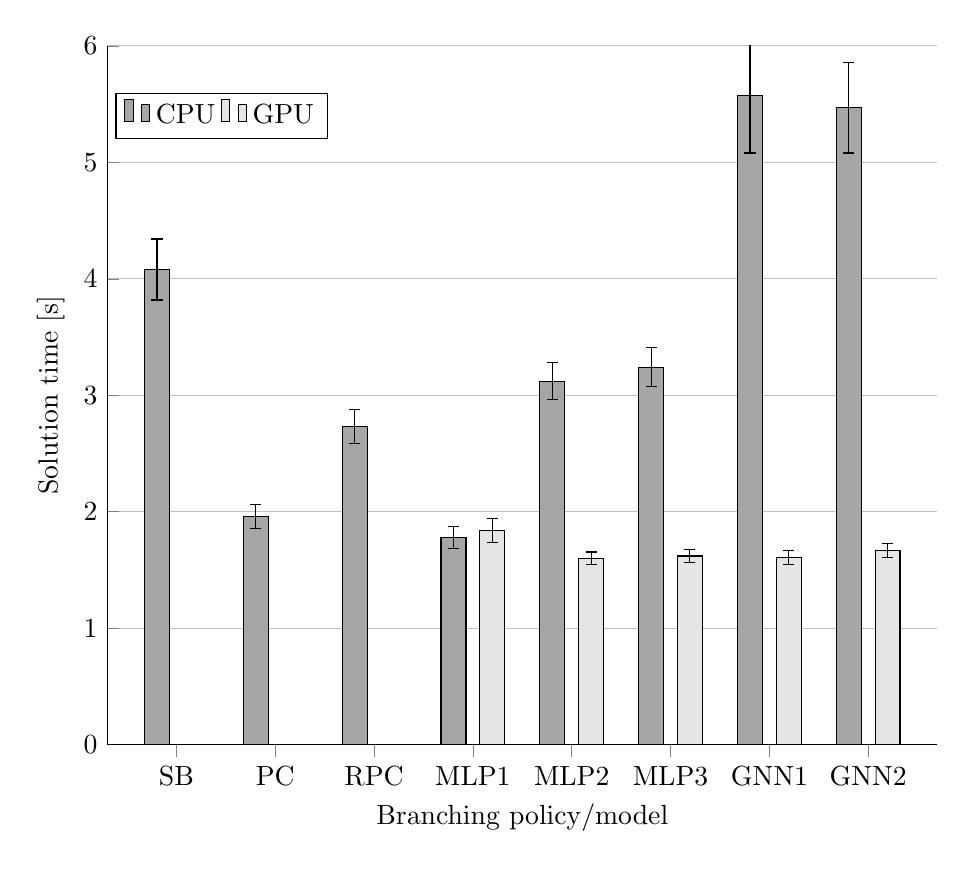
\begin{tikzpicture}
    \begin{axis}[
        width=\linewidth,
        axis x line*=bottom,
        axis y line*=left,
    	ylabel={Solution time [s]},
    	xlabel={Branching policy/model},
    	ymajorgrids=true,
    	ybar=5pt,% configures `bar shift'
    	bar width=9pt,
        xticklabels={SB,PC,RPC,MLP1,MLP2,MLP3,%
		GNN1,GNN2},
		xtick=data,
		%enlarge x limits=0.15,
        %enlarge y limits=0.05,
        %restrict y to domain=0:6
        ymin=0.0,   ymax=6.0,
	    legend style={at={(0.01,0.9)},anchor=west,legend columns=-1}
    ]
    \addplot[color=black,fill=black!35,error bars/.cd,y dir=both,y explicit,]
    coordinates{
       (1,4.08) +-(0.0,0.262)
       (2,1.96) +-(0.0,0.1043)
       (3,2.73) +-(0.0,0.146)
       (4,1.78) +-(0.0,0.0967)
       (5,3.12) +-(0.0,0.159)
       (6,3.24) +-(0.0,0.167)
       (7,5.57) +- (0.0, 0.49)
       (8,5.47) +- (0.0, 0.39)
    };
    %negativ
    \addplot[color=black,fill=black!10,error bars/.cd,y dir=both,y explicit,]
    coordinates {
      %(1,0.9365) +- (0.00587,0.00587)
      %(2,0.1435) +- (0.01737,0.01737)
      (4,1.84) +-(0.0,0.103)
      (5,1.60) +-(0.0,0.0545)
      (6,1.62) +-(0.0,0.0558)
      (7,1.61) +- (0.0, 0.06)
      (8,1.67) +- (0.0, 0.06)
};
    \legend{CPU,GPU}
    \end{axis}
    \end{tikzpicture}
    \caption{Combinatorial Auction test problem mean solution time GPU and CPU.}
    \label{fig:cauctions_bar}
\end{figure}

\begin{figure}[ht]
    \centering
    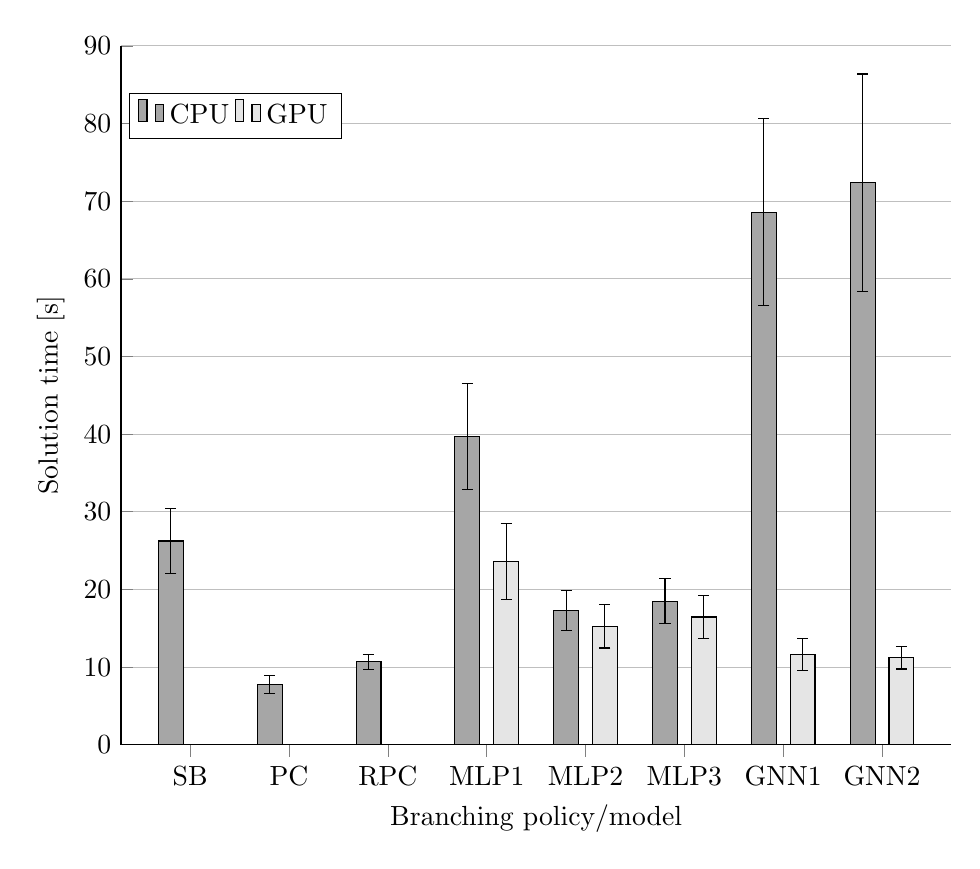
\begin{tikzpicture}
    \begin{axis}[
        width=\linewidth,
        axis x line*=bottom,
        axis y line*=left,
    	ylabel={Solution time [s]},
    	xlabel={Branching policy/model},
    	ymajorgrids=true,
    	ybar=5pt,% configures `bar shift'
    	bar width=9pt,
        xticklabels={SB,PC,RPC,MLP1,MLP2,MLP3,%
		GNN1,GNN2},
		xtick=data,
		%enlarge x limits=0.15,
        %enlarge y limits=0.05,
        %restrict y to domain=0:6
        ymin=0.0,   ymax=90.0,
	    legend style={at={(0.01,0.9)},anchor=west,legend columns=-1}
    ]
    \addplot[color=black,fill=black!35,error bars/.cd,y dir=both,y explicit,]
    coordinates{
       (1,26.23) +-(0.0, 4.19)
       (2,7.78) +-(0.0, 1.18)
       (3,10.68) +-(0.0,0.993)
       (4,39.70) +-(0.0, 6.83)
       (5,17.26) +- (0.0, 2.6)
       (6,18.46) +- (0.0, 2.9)
       (7,68.59) +-(0.0,12)
       (8,72.37) +-(0.0,14)
    };
    %negativ
    \addplot[color=black,fill=black!10,error bars/.cd,y dir=both,y explicit,]
    coordinates {
      %(1,0.9365) +- (0.00587,0.00587)
      %(2,0.1435) +- (0.01737,0.01737)
      (4,23.58) +- (0.0, 4.86)
      (5,15.26) +- (0.0, 2.8)
      (6,16.45) +-(0.0,2.8)
      (7,11.63) +-(0.0, 2.07)
      (8,11.18) +-(0.0, 1.43)
};
    \legend{CPU,GPU}
    \end{axis}
    \end{tikzpicture}
    \caption{Set covering test problem solution time GPU and CPU.}
    \label{fig:set_bar}
\end{figure}


\begin{comment}
    
\begin{figure}
    \centering
    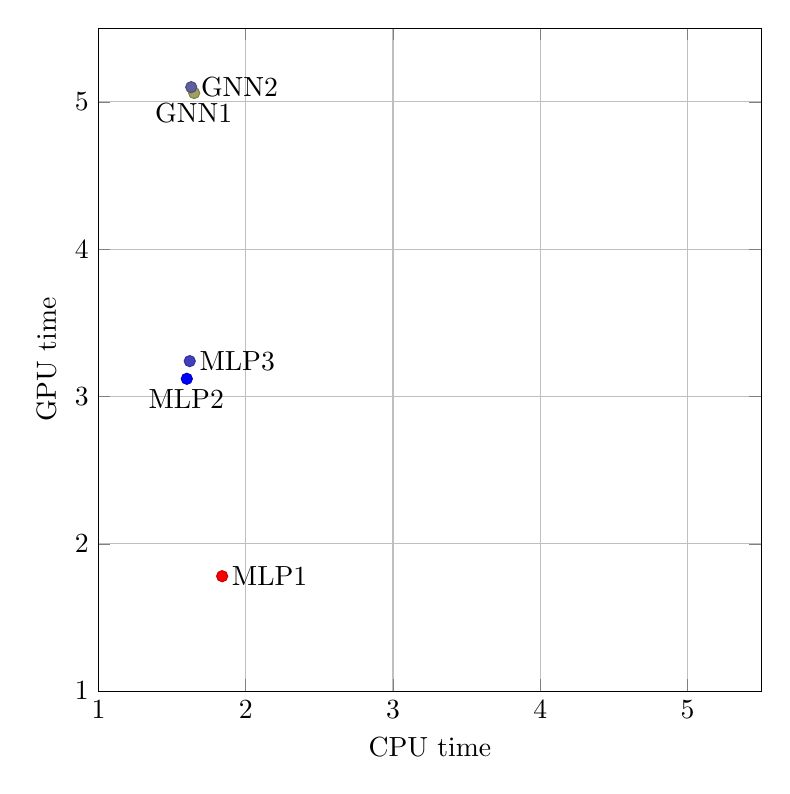
\begin{tikzpicture}
    
      \def\MarkSize{.75em}
      \protected\def\ToWest#1{%
        \llap{#1\kern\MarkSize}\phantom{#1}%
      }
      \protected\def\ToSouth#1{%
        \sbox0{#1}%
        \smash{%
          \rlap{%
            \kern-.5\dimexpr\wd0 + \MarkSize\relax
            \lower\dimexpr.375em+\ht0\relax\copy0 %
          }%
        }%
        \hphantom{#1}%
      }
    \begin{axis}[ xlabel={CPU time}, ylabel={GPU time}, width=10cm, height=10cm, ymin=1.0, ymax=5.5, xmin=1.0,   xmax=5.5, ymajorgrids=true,
    xmajorgrids=true,]v
    \addplot[scatter,mark=*,only marks, point meta=x,nodes near coords*={\data},
    visualization depends on={value \thisrow{dataname} \as \data},] 
    table [x=x,y=y]{
    x       y       dataname
    1.84    1.78    MLP1
    1.60    3.12    \ToSouth{MLP2}
    1.62    3.24    MLP3
    1.65    5.06    \ToSouth{GNN1}
    1.63    5.10    GNN2
    };
    \end{axis}
    \end{tikzpicture}
    \caption{Combinatorial Auction small problem mean solution time GPU and CPU.}
    \label{fig:gpu_cpu}
\end{figure}
\end{comment}


%In Gasse et al. (2019) \cite{gasse2019exact} and Gupta et al. (2020) \cite{gupta2020hybrid}, the models are also evaluated by their performance on larger problem sizes, as a method of measuring the models' ability to generalize.
%This is a time-consuming process, and therefore only a select number of models is used: MLP1, MLP2, and GNN1, as these represent the variations that are shown in \Cref{fig:cauctions_bar} and \Cref{fig:set_bar}.

%The result is shown in \Cref{tab:results_trans_cauction}, where \textit{time} and \textit{nodes} is measured as in \Cref{tab:results1_cauction} and \Cref{tab:results1_set}.
%\textit{completed} is the number of problems where optimality was achieved within the time limit of 45 minutes and is only applicable for the large problem size. 

%GNN1 and MLP2 perform competitively on the \gls{GPU}, while the \gls{MLP} suffers from the consequences of poor variable branching choices, leading to very poor performance. 

% including transfer learning 

\begin{comment}
    
\begin{scriptsize}
\begin{table}[ht]
	\centering
	\begin{tabular}{lrrrrr}
	    \toprule
		&  \multicolumn{2}{c}{Medium} & \multicolumn{3}{c}{Large}\\ \cmidrule(lr){2-3} \cmidrule(lr){4-6} 
		Model & Time (s) & Nodes & Time (s) & Nodes & Completed\\
		\midrule
		FSB &  $158.03$ & $139 $ & 0 & 0 & 0 / 20\\
		PC  &  $26.40 $ & $5429 $ & $410.24 $ & $54923 $ & 20 / 20\\
		RPC &  $20.60 $ & $1692 $ & $\mathbf{214.30} $ & $19069 $ & 20 / 20\\
		\addlinespace
		MLP1\textsubscript{g}  & $260.18$ & $73895$ & $2490.55$ & $424168$ & 6 / 20\\
		MLP2\textsubscript{g} &  $19.20$ & $2875$ & $470.39$ & $53314$ & 20 / 20\\
		GNN1\textsubscript{g} & $\mathbf{15.76}$ & $1628$ & $273.89$ & $25879$ & 20 / 20\\
		\addlinespace
		MLP1\textsubscript{c} &  $667.74 $ & $74891 $ & $9556.22 $ & $463156 $ & 1 / 20\\
		MLP2\textsubscript{c} &  $60.87 $ & $2871$ & $1791.31 $ & $53933 $ & 15 / 20\\
		GNN1\textsubscript{c} & $118.54 $ & $1701 $ & $2197.60 $ & $26470 $ & 14 / 20\\
		\bottomrule
	\end{tabular}
	\caption{Combinatorial auction solving efficiency on larger problem sets.}\label{tab:results_trans_cauction}
\end{table}
\end{scriptsize}
\end{comment}
% time 158.03 \pm 227.58  | nb nodes     139 \pm  187
%MLP1 cpu
%04-24 11:37:37.76] ------ cauctions, large ------
%[04-25 02:04:00.40]  nb nodes     +- 93142 |  time  +- | completed    1
%
% include feature importance

% include solution hists nnodes

